\documentclass[a4paper,twoside]{article}
\usepackage{graphicx}
\usepackage{url}
\usepackage[bf]{caption}

\setlength {\textwidth}{150mm}
\setlength {\captionmargin}{20pt}
\oddsidemargin 5mm
\evensidemargin 5mm

\begin{document}

\title{RealityGrid Generic Steering Client User Manual}
\author{Robert Haines, Mark Riding and Andrew Porter
\\Research Computing Services
\\University of Manchester
\\Oxford Road
\\Manchester
\\M13 9PL
\\United Kingdom}
\date{}

\maketitle

\begin{table}
\begin{center}
\begin{tabular}{r|p{8cm}|c}
\hline\hline
Author & Comments & Date \\
\hline
Andrew Porter & As released with v.1.1 of the RealityGrid steering software. & April 2004 \\
Andrew Porter & Extensions for tabbed steering and additional graphing features. & November 2004 \\
Andrew Porter & As released with v.1.2 of the RealityGrid steering software. & April 2006\\
Andrew Porter & As released with v.2.0 of the RealityGrid steering software. & July 2006\\
Robert Haines & As released with v.3.5 of the RealityGrid steering software. & June 2010\\
\hline\hline
\end{tabular}
\end{center}
\end{table}

\pagebreak

\tableofcontents

\pagebreak

\begin{section}{Introduction}

The RealityGrid Steerer is a generic user interface for performing
computational steering of (computational) jobs which have been
instrumented using the RealityGrid Steering API. This document aims to
give new users an overview of how to use the steerer and to explain
the functionality which it offers.

\end{section}

%--------------------------------------------------------------------

\begin{section}{Configuration}
\label{sec:config}

Several configuration options for the steering client are set by means
of a file, `steerer.conf,' which should be installed in the user's
\texttt{$\sim$/.realitygrid} directory. An example of this file is
shown in figure~\ref{fig:steerer_conf}.  The configuration file
specifies the address of the top-level registry (where the steerer
searches for available jobs to steer when using Web Services) and has
sections for the control of the appearance of the main GUI window and
the frequency with which the steerer polls for status messages.  The
pollingInterval is specified in seconds and has a maximum value of
two. If autoPolling is on then the pollingInterval field only gives
the initial value --- the steering client is free to change it.

\begin{figure}[h]
\begin{verbatim}<?xml version="1.0"?>
<Steerer_config>
  <Registry>
    <!-- location of registry.  If it uses SSL then security.conf must hold
         name of certificate+key file and location of CA certs. -->
    <address value="http://a.machine.ac.uk:30035/Session/regServiceGroup/
regServiceGroup/54351518137034689"/>
    <!-- username is only used when registry is not using SSL -->
    <username value="andy"/>
  </Registry>
  <Polling>
    <!-- whether or not to allow the steering client to control how often
         it polls for new status messages -->
    <autoPolling value="on"/>
    <!-- Initial polling interval in seconds -->
    <pollingInterval value="0.5"/>
  </Polling>
  <Display>
    <showMonParamTable value="on"/>
    <showSteerParamTable value="on"/>
    <showIOTypesTable value="on"/>
    <showChkTypesTable value="on"/>
  </Display>
</Steerer_config>
\end{verbatim}
\caption{An example of the contents of the steerer configuration file.}
\label{fig:steerer_conf}
\end{figure}

As of version 2.0 of the RealityGrid Steering Library, the use of
OGSI-based Grid Services has been superseded by WSRF-based Web
Services.  As part of this change, both the Registry and the Steering
Web Service (SWS) itself may be secured using both SSL and a
WS-Security-based username/password scheme. If SSL is being used then
the steering client obtains the location of the certificates of the
Certificate Authorities that it trusts and the file containing the
user's private key and certificate from the `security.conf' file
(figure~\ref{fig:security_conf}). The file containing the user's key
{\em and} certificate may be constructed by simply concatenating the
two separate pem-format files that hold the two items:
\begin{verbatim}
  cat userCert.pem > userCertAndKey.pem
  cat userKey.pem >> userCertAndKey.pem
\end{verbatim}
Like steerer.conf, the security.conf file should be installed in the user's
\texttt{$\sim$/.realitygrid} directory.

\begin{figure}
\begin{verbatim}
  <?xml version="1.0"?>
  <Security_config>
    <caCertsPath value="/etc/grid-security/certificates"/>
    <privateKeyCertFile value="/home/myname/.globus/usercertandkey.pem"/>
  </Security_config>
\end{verbatim}
\caption{An example of the contents of the security configuration file.}
\label{fig:security_conf}
\end{figure}

\end{section}

%--------------------------------------------------------------------

\begin{section}{Starting the Steerer}

\begin{subsection}{Launching}

Run the steering application by executing the command \texttt{steerer}
at the command prompt (assuming that it is in your path). You will be
presented with a simple start-up screen as shown in
figure~\ref{fig:startup_screen}.


\begin{figure}
\centerline{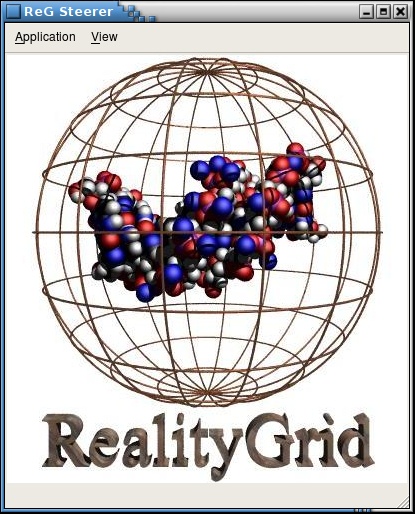
\includegraphics{startup_screen.png}}
\caption{Steerer start-up screen}
\label{fig:startup_screen}
\end{figure}

\end{subsection}

%---------------------------

\begin{subsection}{The Application menu}


\begin{figure}
\centerline{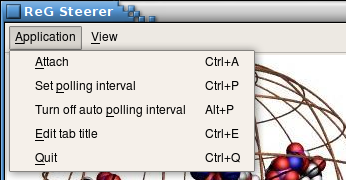
\includegraphics{app_menu.png}}
\caption{The main steering client menu}
\label{fig:steerer_menu}
\end{figure}

The Application menu (figure~\ref{fig:steerer_menu}) has five
options\footnote{Note that on Mac OS X the \texttt{Cmd} and
  \texttt{Option} keys are used instead of \texttt{Ctrl} and
  \texttt{Alt} respectively. Additionally, the Quit option is in the
  `Steerer' menu rather than the `Application' menu in line with Mac
  OS X convention.}:
\begin{itemize}
\item Attach: attach to a steerable job. The options with which the
  steering library has been compiled with will determine how the
  connection is made. Shortcut Ctrl+A;
\item Set Polling Interval: set how often (in seconds) the
steerer polls the computational job. Shortcut Ctrl+P;
\item Turn on/off auto polling interval: toggle whether or not
to allow the client to automatically adjust the polling
interval. Shortcut Alt+P;
\item Edit the title of the current tab. Shortcut Ctrl+E;
\item Quit: Quits the application. Shortcut Ctrl+Q.
\end{itemize}

The Polling Interval is an important parameter since it controls how
often the steerer checks for status messages from an attached
application.  If the steerer fails to `keep up' with the application
then status messages will be lost which may result in strange
behaviour.  For applications that generate many status reports per
second, the value of the \texttt{STEERING INTERVAL} steerable
parameter of that application should be increased in order to reduce
the frequency with which it generates status reports. (This steerable
parameter is automatically generated by the steering library and is
thus available for all applications that use the RealityGrid steering
library.)  Allowing the steering client to automatically configure the
polling interval is recommended although users should still ensure
that applications are not generating more than about two status
messages per second.

Editing the tab title is particularly useful when the steering client
is attached to multiple applications (see
section~\ref{sec:multiple_sims}).  It allows the user to give more
meaningful names to the tabs being used to display information from
each application.  (By default, each tab title is either the address
of the Web Service representing the application or the directory from
which message files are being read, depending on whether SOAP-based or
file-based steering is being used, respectively.)

\end{subsection}

\begin{subsection}{Attaching to a steerable job}

\begin{figure}
\centerline{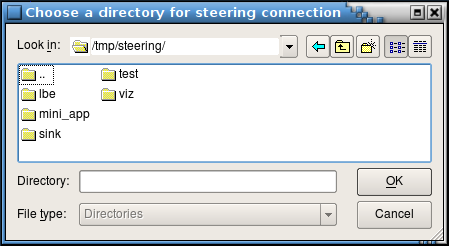
\includegraphics{dir_browser.png}}
\caption{Browser dialog for choosing a directory for steering communication}
\label{fig:dir_browser}
\end{figure}

Selecting `Local Attach' from the Steerer menu will open a file-system
browser (figure~\ref{fig:dir_browser}) that allows you to choose the
directory to use for communication with the application that you wish
to steer.  This directory must match that passed to the application by
way of the REG\_\-STEER\_\-DIRECTORY environment variable.  On
pressing OK the main RealityGrid Steerer window should be displayed.
Should the steerer fail to find an application to attach to then the
Steerer start-up screen will have a `Failed to attach' message
displayed at the bottom of it.  If this occurs then check that you
have selected the correct directory and that the application is
actually up and running.

\begin{figure}
\centerline{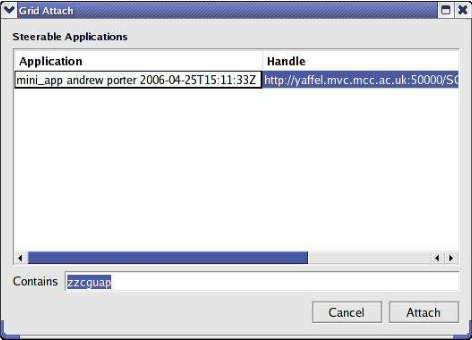
\includegraphics{grid_attach.png}}
\caption{Grid Attach dialog}
\label{fig:grid_attach}
\end{figure}

Selecting `Grid Attach' will bring up a small dialog box
(figure~\ref{fig:grid_attach}) listing all available RealityGrid
applications and their addresses (handles) in a table.  (This
information is obtained by querying the registry specified in the
configuration file --- see section~\ref{sec:config}.) Entries in the
Handle column are fully editable.  By selecting an entry in the table
and clicking on the Attach button, a Steerer is created for the chosen
application. Should the attach fail then check that the handle you've
specified is correct and that the application you are attempting to
connect to is up and running.  (A good way of doing the latter is to
check that the \texttt{sws:machineName} ResourceProperty of the
Steering Web Service has been set.  If it hasn't then the job
has failed to contact the Web Service and you should look at its
stderr output.)

It is also possible (on Linux/UNIX systems) to specify the handle to
connect to on the command line when launching the steerer.

\end{subsection}
\end{section}

%------------------------------------------------------------------

\begin{section}{The Main Window}

\begin{figure}
\centerline{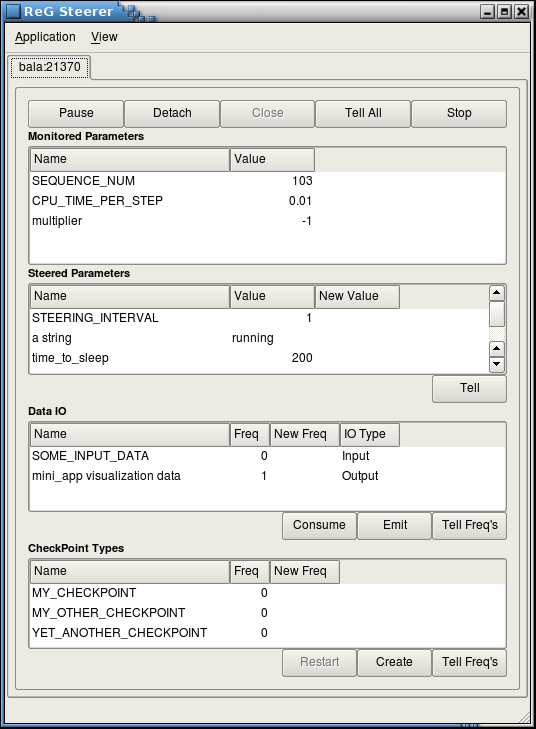
\includegraphics{main_sockets.png}}
\caption{Steerer main window in direct-steering mode}
\label{fig:main_socks}
\end{figure}

Once the steerer has successfully attached to a job, the main window
is displayed.  When direct (sockets-based) steering is being used, this
should appear something like the one in figure~\ref{fig:main_socks}.
The Main Window is split into five conceptual sections:
\begin{itemize}
\item Control Buttons
\item Monitored Parameters
\item Steered Parameters
\item Data IO
\item CheckPoint Types
\end{itemize}
The last four of these each have a table associated with them, as
shown in figure~\ref{fig:main_socks}.  The user can choose to hide one
or more of these tables via the View menu shown in
figure~\ref{fig:view_menu}.  By default, all four tables are displayed
once the steerer has successfully attached to a job.  However, this
may be changed by editing the configuration file
(section~\ref{sec:config}).

\begin{figure}
\centerline{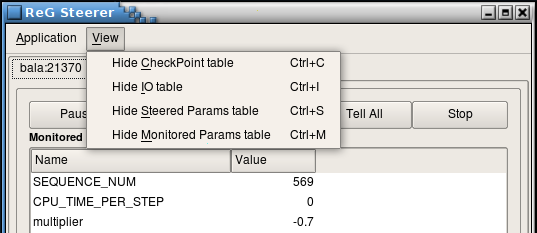
\includegraphics{main_view_menu.png}}
\caption{The View menu on the main window}
\label{fig:view_menu}
\end{figure}

%------------------------

\begin{subsection}{Control Buttons}
\label{sec:control_btns}

The Control Buttons panel manages overall control of the steerable
job's state. Different buttons will be greyed out and unavailable
depending on a job's state; for instance, jobs that are not running
cannot be stopped.  The following buttons are always displayed in the
panel:
\begin{itemize}
\item Pause/Resume: pauses a running job/resumes a paused job;
\item Detach: detaches the steerer from the job, \textit{leaving the
job running};
\item Close: closes the main window of the steerer, returning to the
startup screen;
\item Tell All: causes the steerer to pass any user updated
parameters to the job, see section~\ref{sec:steered_params}.
\item Stop: ends the job;
\end{itemize}

\end{subsection} % Control Buttons

%-----------------------------

\begin{subsection}{Monitored Parameters}
\label{sec:mon_params}

The Monitored Parameters table lists parameters which are exposed by
the steerable job, but may not be changed by the steerer. An example
of a monitored parameter for a simulation job might be wall-clock time
per simulation step. Such a parameter is changed only by the steered
application itself, not the user.

The Steerer allows graphs to be drawn of the history of both monitored
and steerable parameters. By right clicking on a monitored parameter,
a context menu appears allowing the user to select a `Draw History
Graph' option (figure~\ref{fig:hist_graph_context_menu}). If one or
more History Plots are already open then this menu also includes an
option to add a plot of this parameter to one of them. For more
details see section~\ref{sec:hist_graphs}.

\begin{figure}
\centerline{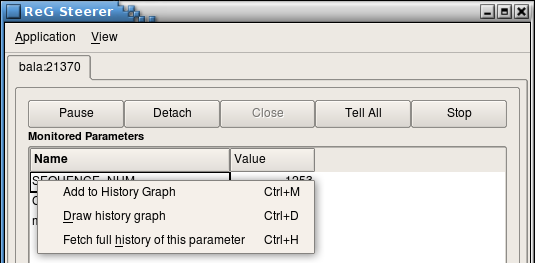
\includegraphics{hist_plot_context_menu.png}}
\caption{Draw History Graph context menu option}
\label{fig:hist_graph_context_menu}
\end{figure}

\end{subsection} % Monitored Parameters

%-----------------------------

\begin{subsection}{Steered Parameters}
\label{sec:steered_params}

The Steered Parameters table contains a list of all steerable
parameters exposed by the current job. The first column, `Name,' lists
the names of each of the parameters (as specified when they were
registered with the steering library), the second, `Value,' shows the
current value for each parameter, and the third, `New Value,' allows
the user to enter new values. Hovering the mouse over an entry in the
third column brings up a tool tip showing the minimum and maximum
allowable values for that parameter, as shown in
figure~\ref{fig:limits_tool_tip}.  If the steerable parameter is a
string then the maximum allowable value gives the maximum length of
the string.

New values are only propagated to the running job once the entry has
been completed (by pressing Enter or leaving the cell via the cursor
keys) and the `Tell' button is clicked. When this happens the entries
in the `Value' column are updated to reflect the new values, and any
entries in the `New Value' column are cleared. This action is also
performed if the user clicks the `Tell All' button in the Commands button
panel.  Note that the entries in the `Value' column are only updated
upon confirmation from the application --- this thus provides
confirmation that it has received the instruction(s).

\begin{figure}
\centerline{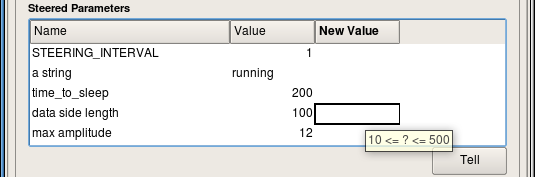
\includegraphics{limits_tool_tip.png}}
\caption{Steered Parameters tool tip showing the limits on a steered
parameter (``data side length'' in this case).}
\label{fig:limits_tool_tip}
\end{figure}

\end{subsection} % Steered Parameters

%-----------------------------

\begin{subsection}{Data IO}

The Data IO table lists all data input and output channels supported
by the current job. The `Name' column lists the name of each channel,
the `Freq' column lists how often data is written to or read from the
channel (in time steps), the editable `New Freq' column allows the
user to specify a new frequency for each item, and the `IO Type'
column indicates whether the channel is for input or output.  Each
individual entry is either an input or an output, not both. As with
the steered parameters table, any changes are not propagated to the
current job until either the `Tell Freq's' button or the `Tell All'
button in the Commands button panel is clicked.

It is possible to manually request that data be emitted/consumed, in
addition to the automatic events. To do so, select (click on) an entry
in the table, and click the `Consume' or `Emit' button at the right
of the table. Only one of the buttons will be available for each
entry, depending on whether the data channel is for input or output.

\end{subsection} % Data IO

%-----------------------------

\begin{subsection}{CheckPoint Types}

The CheckPoint Types table lists the types of checkpoint that the
running job supports. There can be many instances (checkpoints) of
each checkpoint type, and a job may expose several checkpoint types
which differ in the parameters and data values they record. It is expected
that the majority of jobs will only need a single type of checkpoint.

The `Name' column lists the names of each checkpoint type, the `Freq'
column lists the frequency with which checkpoints are automatically
taken (in time steps), and the editable `New Freq' column allows the user
to enter new values for a checkpoint's frequency. As with the Steered
Parameter values, new frequency values are only propagated to the
running job when either the `Tell Freq's' button or the `Tell All'
button in the Commands button panel is clicked.

There are slight differences in the steerer main window depending on
whether local (file-based) or remote steering (using the web-service
framework) is being performed.

%--------------------------

\begin{subsubsection}{Checkpointing with local steering}

Checkpoints (checkpoint type instances) can be created or used to
perform a restart by means of the `Create' and `Restart' buttons to
the right of the main checkpoint table. These buttons will be greyed
out and unavailable by default, only becoming active if an appropriate
checkpoint type has been selected.

After clicking on the Create button for a valid checkpoint type, the
application will be instructed to create a checkpoint instance of the
selected checkpoint type.  After clicking on the Restart button for a
valid checkpoint type, a dialog (figure~\ref{fig:chk_list_dialog}) is
presented listing all of the recorded checkpoint instances for that
type. You can select a checkpoint instance from the list, and instruct
the application to restart from it by clicking on the `Restart'
button. Clicking on `Cancel' quits the dialog without doing anything.

\begin{figure}
\centerline{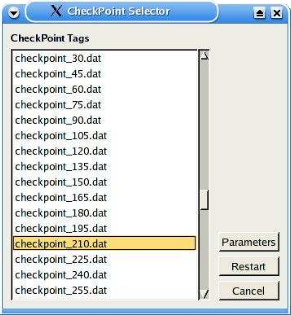
\includegraphics{chk_list.png}}
\caption{CheckPoint Selector dialog}
\label{fig:chk_list_dialog}
\end{figure}

In order to help differentiate between checkpoint instances, it is
possible to inspect the parameters of each by clicking on the
`Parameters' button. This brings up another dialog, which lists the
checkpoint instance's parameters and their values at the time the
checkpoint was taken. It is possible to have several Checkpoint
Parameters Table dialogs open at the same time, so that different
checkpoint instances can be compared and contrasted.  Again, clicking
on the `Cancel' button closes the dialog.

\begin{figure}
\centerline{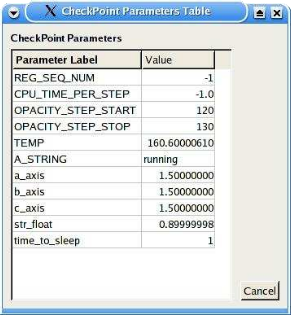
\includegraphics{chk_params.png}}
\caption{CheckPoint Parameters Table dialog}
\label{fig:chk_params_dialog}
\end{figure}

\end{subsubsection}

%--------------------------

\begin{subsubsection}{Checkpointing with remote steering}

When remote steering is in operation, the main window of the steerer
and the way in which a restart is performed is slightly different.
The form of the main window when doing remote steering is shown in
figure~\ref{fig:main_window_grid}.

\begin{figure}
\centerline{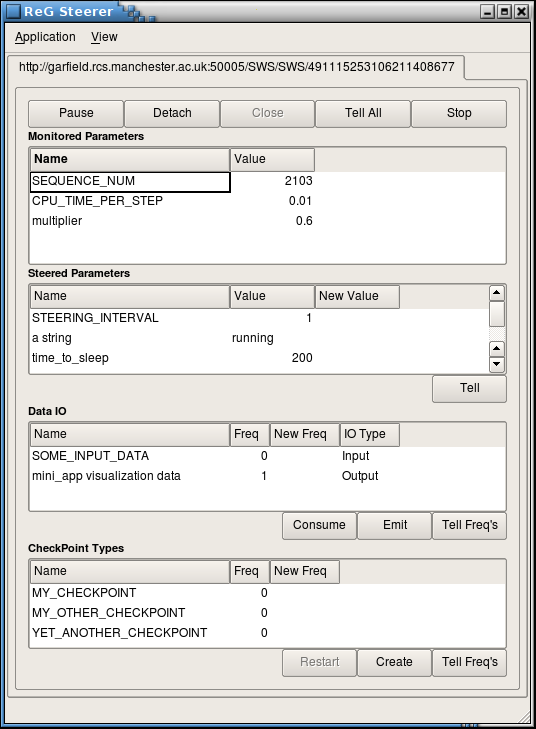
\includegraphics{main_window_grid.png}}
\caption{Steerer main window in remote-steering mode}
\label{fig:main_window_grid}
\end{figure}

A checkpoint is still created by selecting the appropriate checkpoint
type from the checkpoint table and clicking the `Create' button.
However, the `Restart' button is now located in the panel at the top
of the window --- this is because it is no longer necessary to select a
checkpoint type before pressing it.  Instead, on pressing `Restart,'
the user is prompted to enter the Grid Service Handle of a suitable
checkpoint.  How the user obtains this GSH is beyond the scope of this
document since it relies upon the user browsing a checkpoint tree
(using either a web interface or some tool such as the RealityGrid
launching wizard).

\end{subsubsection} % Checkpointing with remote steering

\end{subsection} % CheckPoint Types
\end{section} % Main window

%--------------------------------------------------------------

\begin{section}{Parameter History Graphs}
\label{sec:hist_graphs}

The steerer allows the user to track the changes in both monitored and
steerable parameters by means of 2D plots.  This functionality is
accessed by right-clicking on a parameter in either the Monitored or
Steerable Parameters tables on the main window.  Selecting the `Draw
History Graph' option from the resulting context menu
(figure~\ref{fig:hist_graph_context_menu}) causes a dialog to appear allowing
the user to choose which parameter to plot the chosen one against.
(Parameters are specified using the label with which they were
registered.)  Once the user has completed this dialog a new window
appears containing a 2D line plot of the selected parameter's
history. An example of a plot is shown in
figure~\ref{fig:eg_param_hist_plot}.  The graph is constructed simply
by connecting adjacent ordinates with straight lines --- no fitting is
performed.

\begin{figure}
\centerline{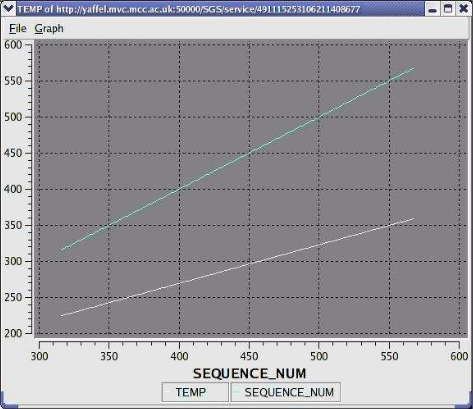
\includegraphics{hist_plot_2curves.png}}
\caption{Example Parameter History Graph}
\label{fig:eg_param_hist_plot}
\end{figure}

The data that is plotted is that collected whilst the steering client
has been attached to the job. If the user wishes to see the history of
a parameter since the beginning of the job then they must right-click
on the parameter's entry in the Monitored/Steerable Parameters table
and select the `Fetch full history of this parameter' option.  Note
that if a parameter is plotted against anything other than the
SEQUENCE\_NUM then the user must also request that the full history of
the parameter being used as the abscissa be fetched.

The history of more than one parameter may be displayed in a single
graph.  Once one or more history graphs are already open, the
parameter context menu has an additional `Add to History Graph'
option. On selecting this option the user must click on the {\em canvas} of
the graph to which they wish to add the plot.

There are two menus available in a History graph window
(figure~\ref{fig:param_hist_menus}), the File menu, and the Graph
menu. The File menu has four options:
\begin{itemize}
\item Print: requests a print-out of the image portion of the window.
Shortcut Ctrl+P;
\item Save: saves the image portion of the window to disk. Shortcut Ctrl+S;
\item Save data: saves the raw data to ASCII file (pops up a file browser).
Shortcut Ctrl+t;
\item Close: closes the window. Shortcut Ctrl+C.
\end{itemize}
The Graph menu has nine options:
\begin{itemize}
\item Auto Y Axis: allows the application to automatically determine
limits for the y-axis. This menu item toggles on and off.
Shortcut Ctrl+A;
\item Define Y upper-bound: if Auto Y axis is not selected, this
menu item becomes available. By selecting it, a dialog appears
(see below) allowing you to enter an upper bound for the Y axis.
If Auto Y Axis is reselected, then this value is ignored.
Shortcut Ctrl+U;
\item Define Y lower-bound: as `Define Y upper-bound', but for
the lower bound. Shortcut Ctrl+L;
\item Toggle use of Log Y axis: switches between linear and
logarithmic axis.  Manual limits cannot be set for the logarithmic
axis and therefore those options will be disabled as appropriate.
Shortcut Ctrl+O;
\item Auto X Axis: allows the application to automatically
determine limits for the x-axis. This menu item toggles on and
off. Shortcut Alt+A;
\item Define X upper-bound: as for Y upper bound. Shortcut Alt+U;
\item Define X lower-bound: as for Y lower bound. Shortcut Alt+L;
\item Toggle use of Log X axis:	as for Log Y axis. Shortcut Alt+O;
\item Toggle display of symbols: enables/disables the display of
symbols at data points. Shortcut Ctrl-D.
\end{itemize}
Symbols are displayed by default if the graph is of an appropriate
scale --- if resolution does not permit then they are automatically
hidden.

\begin{figure}
\centerline{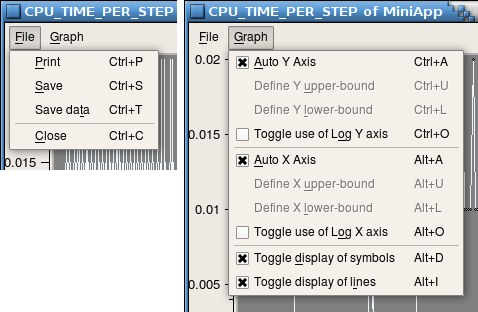
\includegraphics{hist_plot_menus.png}}
\caption{The File and Graph menus of the Parameter History Graph window}
\label{fig:param_hist_menus}
\end{figure}

Note that the steering client automatically logs the values of all
monitored and steerable parameters (irrespective of whether they are
being plotted) and therefore if it is connected to a running
simulation for an extended period it may accumulate a considerable
amount of data.  Displaying a history plot of a large data set
obviously uses some computational resource, particularly if the plot
is being updated frequently.  It may therefore become necessary (in order to
maximise the responsiveness of the steering client) to close history plots
while not in use if the steering client is being used to
continuously monitor long runs.

\end{section} % Parameter History Graphs

%--------------------------------------------------------------

\begin{section}{Steering multiple simulations}
\label{sec:multiple_sims}

The steering client is capable of steering a number of simulations
simultaneously.  These simulations may be local, remote or a mixture
of both.  Connecting to additional simulations is straightforward; use
the `Local Attach' or `Grid Attach' options and proceed as normal.  When
the client is successfully attached to a second application then a
second tab will be added to the main window, as shown in
figure~\ref{fig:tabbed}.

\begin{figure}
\centerline{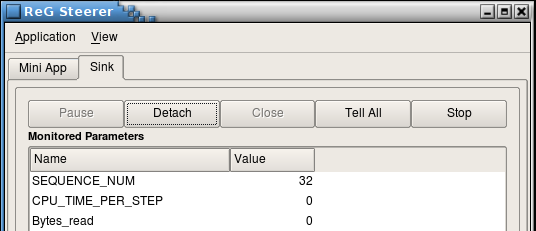
\includegraphics{tabbed_steerer.png}}
\caption{Tabbed steering client connected to two simulations.}
\label{fig:tabbed}
\end{figure}

Initially, the tab is labelled with either the directory or address of the
SWS being used to contact the simulation.  This may be edited by
selecting the `Edit tab title' option from the Steerer menu (shortcut
Ctrl-E).

When the steerer is connected to more than one simulation then
obviously it needs to check for status messages more frequently.  This
must be borne in mind if the user is setting the steerer's polling
interval manually.  However, if the steerer is automatically setting
the polling interval then this is not an issue.  Clearly, there are
practical limits on how many applications the steering client can
connect to simultaneously and these are largely governed by how often
it is possible for the steering client to check for messages.
Although it might be possible to poll for messages very frequently,
this can result in a very unresponsive GUI and therefore the polling
interval must be greater than approximately 0.05 seconds.

\end{section} % Steering multiple simulations

%--------------------------------------------------------------

\begin{section}{Acknowledgements}

The RealityGrid Steerer was initially developed by Sue Ramsden and has
been extended, enhanced and supported by Robert Haines, Mark Riding
and Andrew Porter. The steerer makes use of the RealityGrid Steering
API, by Robert Haines and Andrew Porter.

\end{section}

\end{document}
